The SSP1-MOB vision of the future described in \sref{s:results:ssp1-mob} is used in the following sections to synthesise the changes that the mobility paradigm must undergo\footnote{The changes are not ``suffered'' by an autonomous and disconnected system of mobility, but are introduced by all the agents that play a part in it: users, industries, governments, decision makers, researchers, planners, etc.} to reach the desired form. The synthesis is done using backcasting approach, for which an ``intermediate step'' is presented in \ssref{ss:results:backcasting-2050-intermediate-step}, by showing the state of the same fundamental SSP1-MOB variables, but for the year 2050. The changes between the 2100 and 2050 storylines, along with the ones between the 2050 narrative and the current situation (2017) are then provided in \ssref{ss:results:backcasting-the-path}

\subsection{SSP1-MOB 2050: an intermediate step to sustainable mobility}
\label{ss:results:backcasting-2050-intermediate-step}
In order to ease the backcasting process in \ssref{ss:results:backcasting-the-path}, an intermediate step or ``state'' is developed herein to stress the changes in the trends identified in \ssref{ss:results:ssp1-mob-development}. To summarise the state of the variables and trends, already presented for SSP1-MOB, in the year 2050, a comparison table is provided in \tref{t:ssp1-mob-2050-narrative-thesis}. Both 2100 and 2050 desired states for sustainable mobility are shown side-by-side.
%
\begin{landscape}
{\scriptsize
\begin{longtable}{p{2.5cm}p{3.5cm}p{6cm}p{6cm}}
\caption[Comparison of SSP1-MOB qualitative variables (2050 vs 2100)]{Comparison of qualitative variables underlying to the 2050 and 2100 SSP1-MOB narratives.}\\
\toprule
& & \multicolumn{2}{l}{Trend or status}\\
\cmidrule(l){3-4} Category & Variable or feature & SSP1-MOB 2050 & SSP1-MOB 2100\\
\midrule
\endfirsthead
\caption*{(\emph{continued}) Comparison of SSP1-MOB qualitative variables (2050 vs 2100)}\\
\toprule
& & \multicolumn{2}{l}{Trend or status}\\
\cmidrule(l){3-4} Category & Variable or feature & SSP1-MOB 2050 & SSP1-MOB 2100\\
\midrule
\endhead
\bottomrule
\endfoot
\bottomrule
\endlastfoot
\label{t:ssp1-mob-2050-narrative-thesis}
\textit{Development scenario} & Societal sustainability awareness & Medium & High \\*
 & Travel demand per capita (pkm/yr) & Similar to the baseline (2017) & Lower than the baseline (2017) \\*
 & Total travel demand (pkm/yr) & Higher than the baseline (2017) & Higher than the baseline (2017) \\*
 & Consumption patterns & Lower consumption levels in HICs, increased consumption in LICs & Less carbon (travel) intensive consumption; lower consumption levels \\*
 & Carbon intensity & Medium; power grid is increasingly decarbonized, but not completely & Low; the system is as decarbonized as possible (electrification) \\*
 & IT access & Widespread in HICs; increasing use of IT services for teleworking, car sharing, intermodal travel, \ldots & Widespread, high speed and capacity networks; IT services for teleworking, car sharing, intermodal travel, \ldots \\\addlinespace
\textit{Land use (urban development)} & Urban density & Medium-high and increasing & High (higher than 2017 baseline) \\*
 & Land use patterns & Mixed-use development paradigm & Mixed-use development paradigm \\*
 & Economic centralisation & High; big cities accumulate a big share of the activity & Medium; cities are hotspots, but jobs are spread amongst them \\*
 & City sizes & Medium to large; megacities and (sub)urban sprawl beginning to shrink & Medium; avoidance of megacities or (sub)urban sprawl \\ \addlinespace
\textit{Travel modes share} & Intermodal travel & Facilitated, but still not common & Facilitated, high acceptancy and usage \\*
 & Public transport (rail, bus, aviation) & Increasing demand supply; higher than the baseline (2017) & Majority of demand supply; much higher than the baseline (2017) \\*
 & Automobility (private vehicles) & Lower than the baseline (2017) & Still relevant, but much lower than the baseline (2017) \\*
 & Slow modes (walking and cycling) & Moderate increase compared to baseline (2017) & Higher than the baseline (2017) \\ \addlinespace
\textit{Cultural perception} & Mobility & Accessibility as a focus, managed, reasonable travel time, integrated & Accessibility, local in scale, slowed down, managed, reasonable travel time and reliability, integrated \\*
 & Public transport & Public mobility as an affordable and accessible service & Public mobility as a reliable, comfortable, enjoyable and accessible service \\*
 & Automobility & Automobility fills accessibility gaps; symbolic status decreasing & Automobility as a utility to serve a special need \\
\textit{Public transport} & Reliability & Medium (higher than the baseline) & High \\*
 & Consumer cost & Low & Low \\*
 & Accessibility & Medium-high & High \\*
 & Safety & High & High \\*
 & Public transport infrastructure investments & High and continuous & High and continuous \\ \addlinespace
\textit{Automobility} & Reliability & High & High \\*
 & Consumer cost & Medium & High \\*
 & Accessibility & High & High (especially in rural or remote areas) \\*
 & Safety & Medium (especially Low Income Countries) & High (higher risk than public transport) \\*
 & Automobility infrastructure investments (roads, fuel stations, etc.) & Medium; maintenance dominates in HICs; capacity increased in LICs & Low to medium; maintenance covers the majority of the investments; capacity is not increased \\ \addlinespace
\textit{Fuel technology} & Automobiles & Battery electric vehicles and hybrids for short-medium ranged trips; biofuelled for long range & Battery electric vehicles for short-medium ranged trips; hydrogen fuelled for long range \\*
 & Rail & Full electrification of the network & Full electrification of the network \\*
 & Bus & Hybrid, or biofuelled & Electric or hydrogen-fuelled \\*
 & Aviation & Renewable biofuels & Renewable biofuels
\end{longtable}
}
\end{landscape}
%
\begin{figure}
\centering
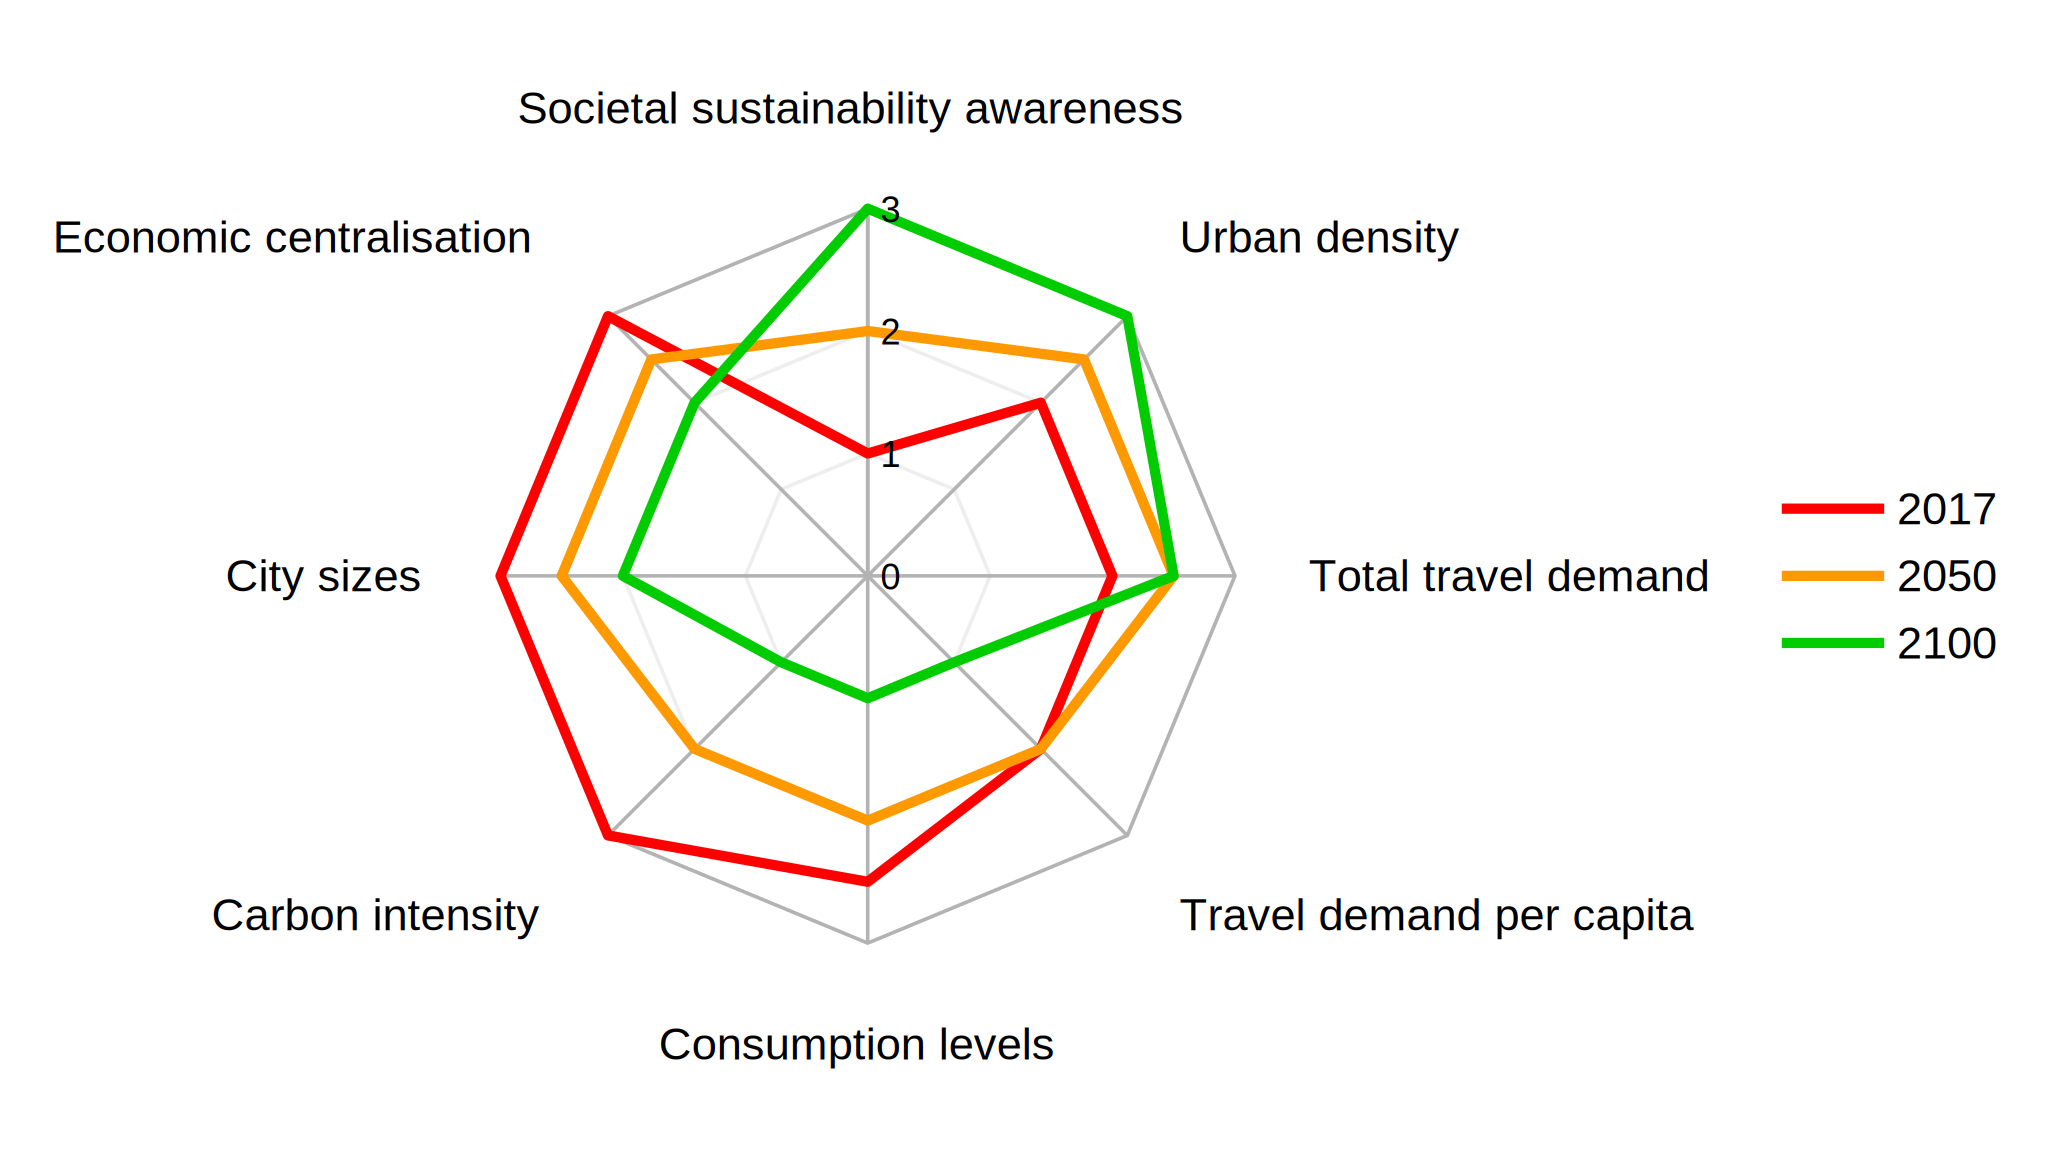
\includegraphics[width=0.7\linewidth]{figures/radar_development-scenario}
\caption[Shifts in development and land-use patterns in SSP1-MOB.]{Radar graph showing the shifts in development trends and land-use patterns found in SSP1 and SSP1-MOB for the years 2100, 2050 and 2017 (baseline). Values are given to the qualitative variables: 3 for high, 2 for medium and 1 for low.}
\label{fig:results:radar_development-scenario}
\end{figure}
%
\begin{figure}
		\centering
  \begin{subfigure}{0.45\textwidth}
    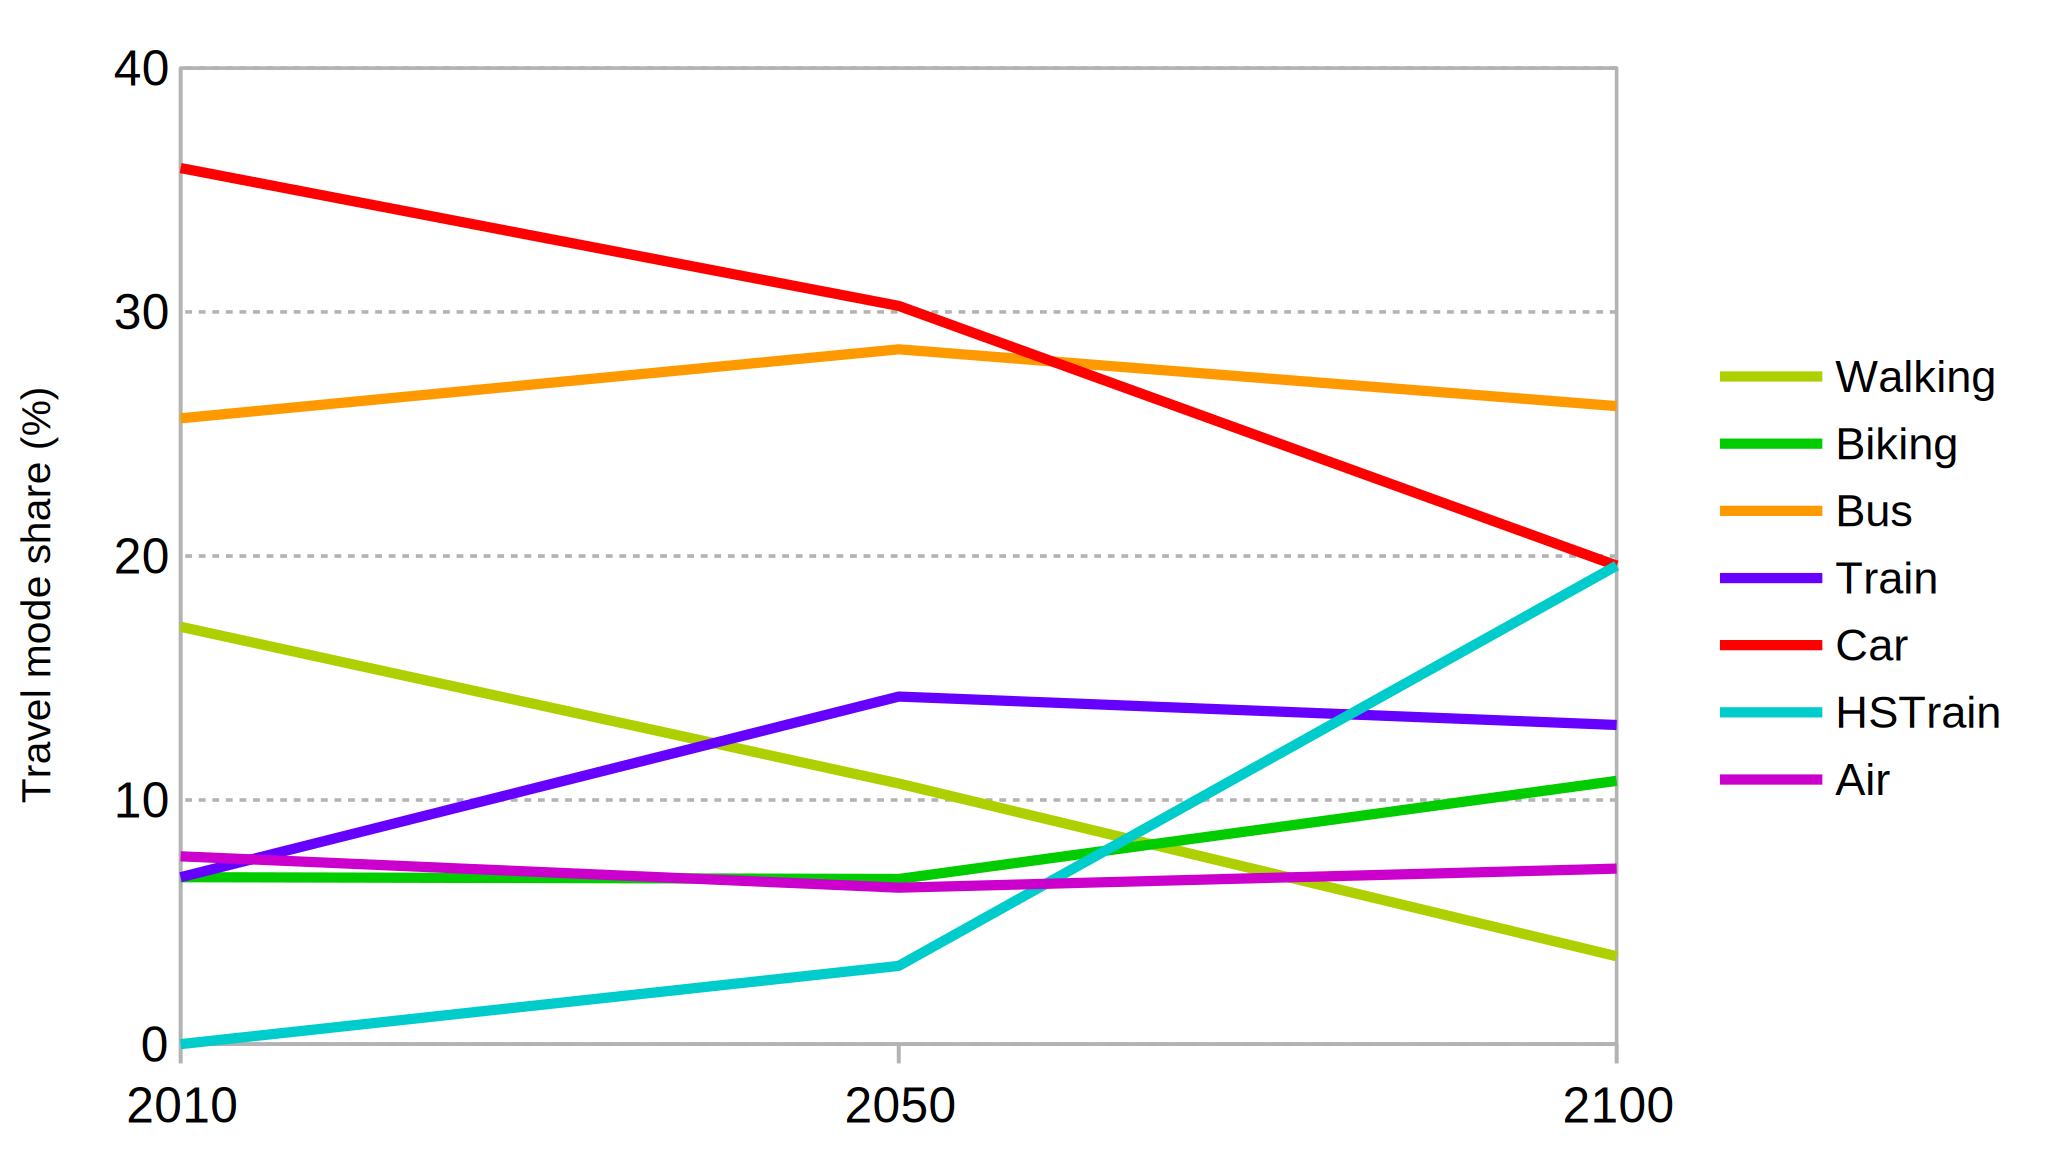
\includegraphics[width=\linewidth]{figures/line_travel-demand-shares.pdf}
    \caption{}
    \label{fig:results:line_travel-demand-shares}
  \end{subfigure}
  \begin{subfigure}{0.45\textwidth}
    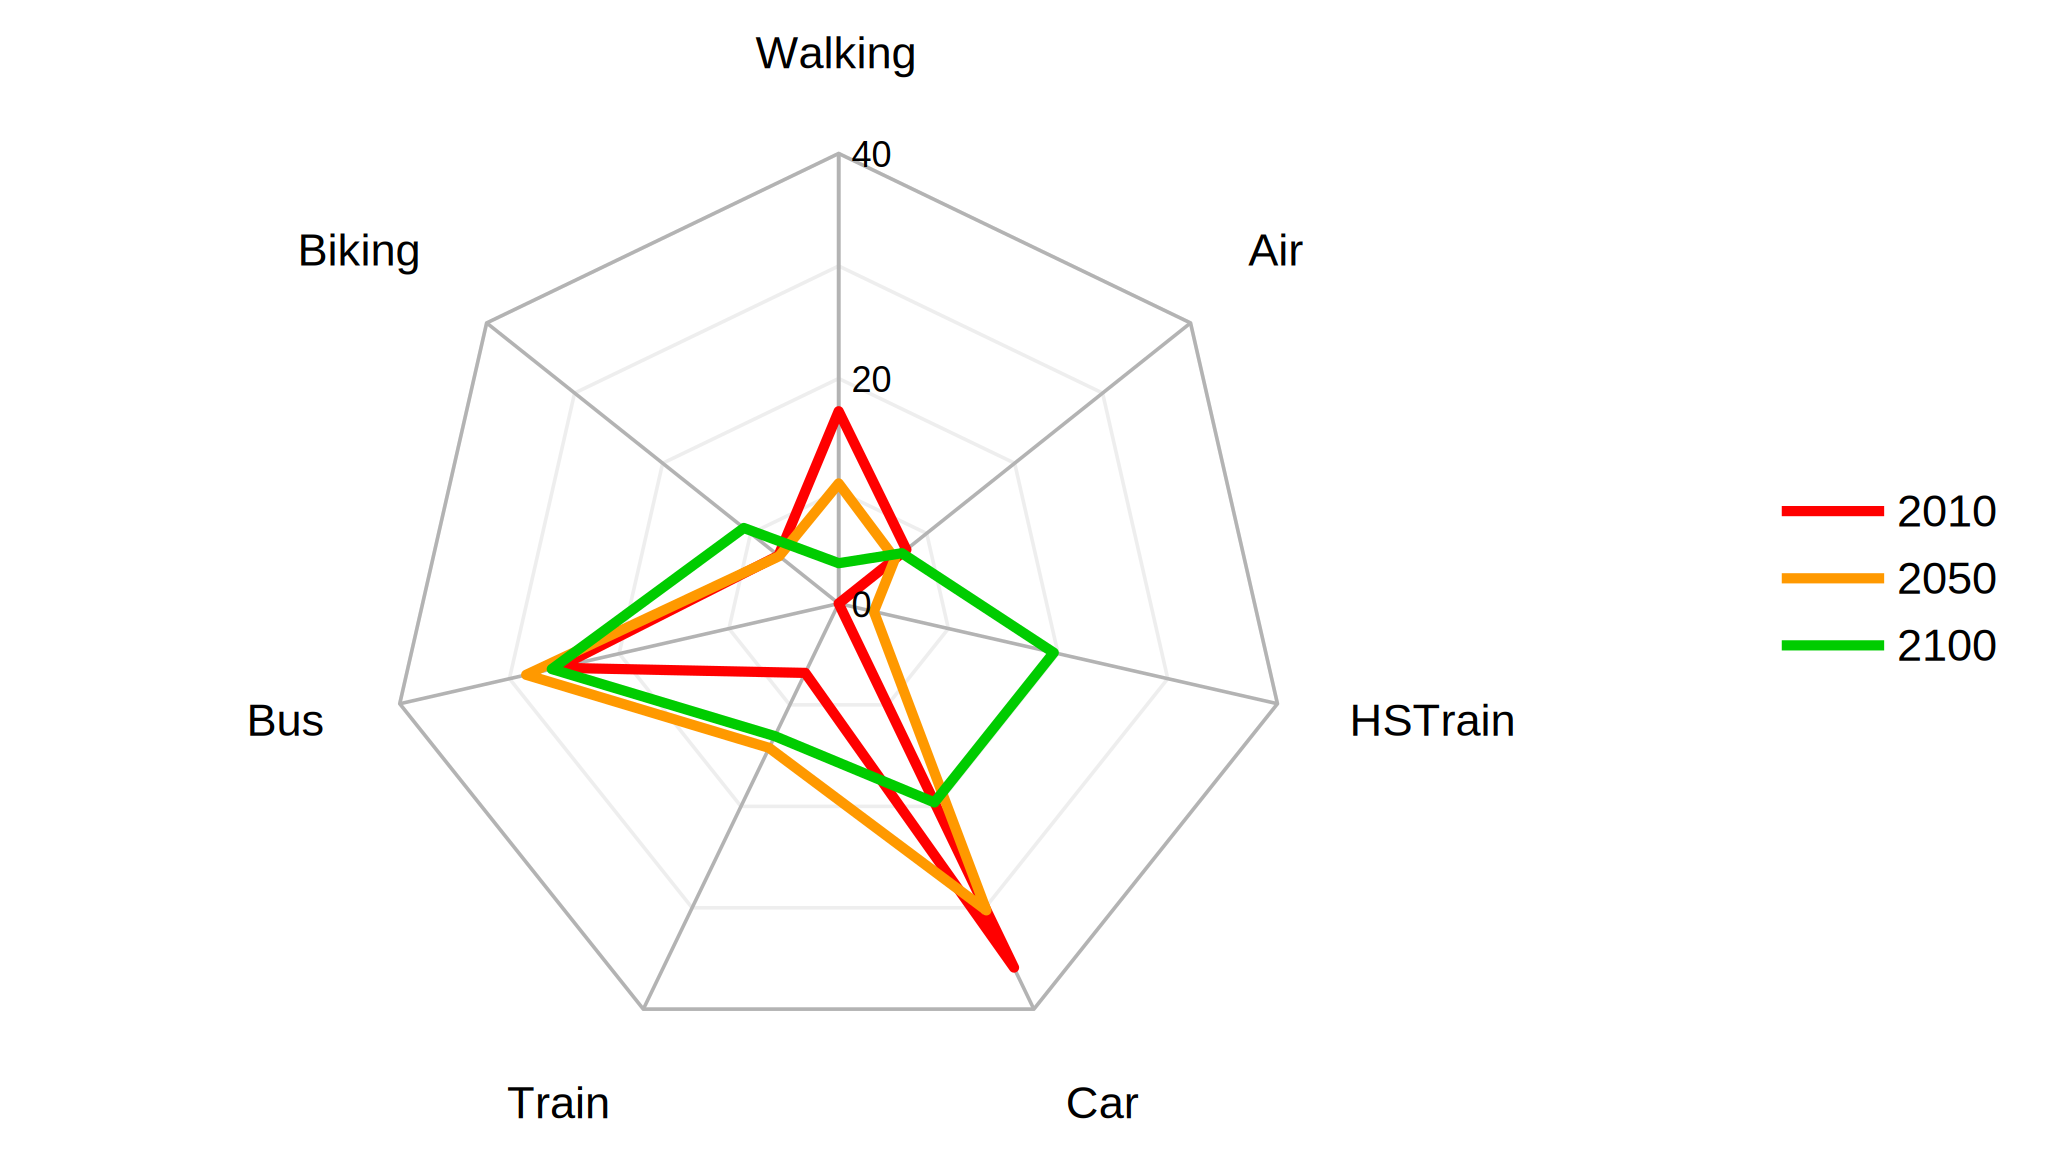
\includegraphics[width=\linewidth]{figures/radar_travel-demand-shares.pdf}
    \caption{}
    \label{fig:results:radar_travel-demand-shares}
  \end{subfigure}
  \caption[Evolution and comparison of travel demand shares in SSP1-MOB.]{Evolution (a) and comparison (b) of total travel demand per transport mode (shares), in percentages, across the SSP1-MOB futures and the 2017 baseline. Note: the demand shares are approximated from the figures provided by \textcite{vuuren2017_Energylanduse} in their quantitative appraisal of the SSP1 scenario.}
\end{figure}


\subsection{The backcasted path to SSP1-MOB}
\label{ss:results:backcasting-the-path}
\todoparagraph{Quick description (table? itemize?) of the changes occurring between the 2050 and 2100 narratives.}
\todoparagraph{Quick description (table? itemize?) of the changes occurring between the 2050 narrative and 2017 baseline.}
\todoparagraph{Explain and contextualise all the backcasted changes: what is the main path to the sustainable future mobility paradigm?}
As already highlighted in the \sref{ss:results:ssp1-mob-paradigm}, one of the key preconditions for the transition to a sustainable mobility paradigm is a change in the \emph{cultural perception} of mobility (how is it understood). This shift of cultural perspective happens not only at the user level, but also at the urban/traffic planner one. \textcite{banister2008_sustainablemobilityparadigm}, drawing from \textcite{marshall2001_challengesustainabletransport}, presents some of the foundation stones of the change to the sustainable mobility paradigm, with which the SSP1-MOB narrative is aligned, and also provides some insight into the cultural contrasts between such a paradigm and the current mobility culture:
%
\begin{enumeratealpha}
\item Instead of speeding up traffic, slowing down traffic is the new target for both users and planners.
\item Streets are seen as a space for urban life, rather than just public spaces occupied by private automobiles only.
\item Social and environmental multicriteria analyses regarding mobility are performed in addition the already dominant economic assessments.
\item Larger travel times become acceptable, in contrast to the current ever accelerating pace of society and mobility.
\item Attention is shifted from vehicles to people: human, personal mobility is the core of the frame, opposed to just vehicle mobility.
\end{enumeratealpha}

\todonote{finish this}